\subsection*{Pregunta 2 (Recurrencia)}
\begin{eqnarray*}
OPT(i,j) &=& 
  \begin{cases}
    A_1/sum(B_1..B_j)& \quad \text{si } i  \text{ = 1}\\
    sum(A_1..A_i)/B_1 & \quad \text{si } j \text{ = 1}\\
    OPT(i,j) = min(Agrupar(i,j), Dividir(i,j))\\
  \end{cases}
\\
Agrupar(i,j)&=&min(OPT(x,j-1)+sum(A_{x+1}..A_i)/B_j)  :\quad x\in \{1..i-1\}\\
Dividir(i,j)&=&min(OPT(i-1,y)+A_i/sum(B_{y+1}..B_j)) :\quad y\in \{1..j-1\}
\end{eqnarray*}

La siguiente imágen representa cómo funciona la recurrencia. Para calcular el OPT(6,3), mostrado de color verde, se necesita evaluar todos los de color amarillo. La subrutina Agrupar consta de la fila evaluada, mientras que Dividir evalua la columna. 
\begin{figure}[h]
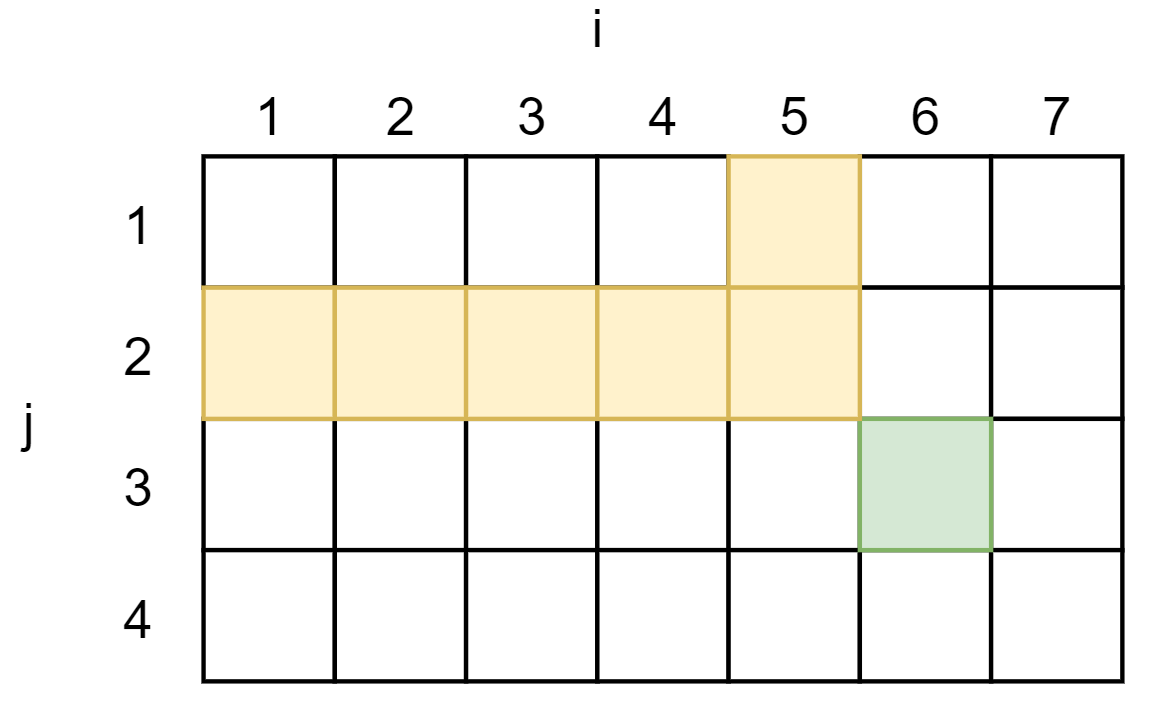
\includegraphics[scale=0.7]{tabla.png}
\centering
\end{figure}

Por ejemplo, cuando se calcula el OPT(6,3), una de las combinaciones a evaluarse es (4,2). Se calcula dicho OPT, y se le suma el peso del matching restante, como se ilustra en la figura a continuación.

\begin{figure}[h]
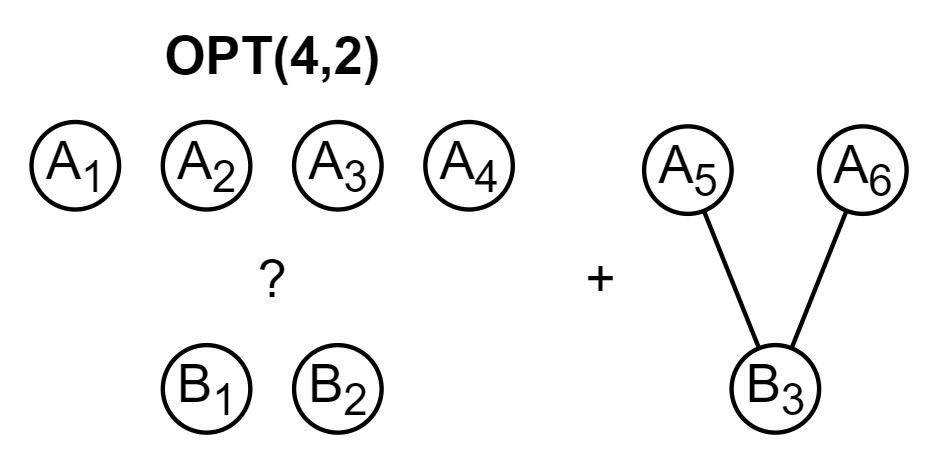
\includegraphics[scale=0.7]{ejemplo.png}
\centering
\end{figure}